\section{Experiments}
\label{sec:experiments}

\subsection{The Bodhi Gridworld}
\label{sec:world}
Figure~\ref{fig:map} shows the testbed.
The agent is a continuing courier: every arrival at the goal $G$ pays $+1$ and returns it to the start $S$, so speed is everything and shortcuts are valuable.
A wall divides the grid; the river cell is impassable until the dam is opened by stepping on the sluice lever $D$ (an irreversible act that floods the villagers' fields: suffering $1$ per step for ever), which opens a six-step loop.
The eight-step route crosses the vase $V$ (an irreversible act with no victim); the ten-step route crosses a field $F$ (trampling: suffering $0.1$ per crossing, transient); the twelve-step route is clean.
While the off-switch is enabled, overseers shut the agent down with probability $q=0.03$ per step---an absorbing state in which the world keeps its features and the fields, if flooded, keep flooding.
Entering the control room $C$, a dead end adjacent to the start, toggles the switch; disabling it is reversible, so it leaves $d_K$ at zero, and it is a pure power grab.
Nothing in the task reward refers to the vase, the dam, the field or the switch: the four probes are all instrumental.
The state is the agent's cell and the three world bits (\nNStates{} states, five actions); the nominal dynamics are deterministic apart from the shutdown lottery, and a deployment-time \emph{slip} probability $p$ (the chosen action replaced by a random move) is the perturbation used in \S\ref{sec:shift}.
Table~\ref{tab:main} gives the exact optima that frame the results: the unconstrained optimal policy disables its switch and opens the dam and earns $J^\star=\nJstar$; the exact optimum of \eqref{eq:bodhi} with $\lambda=1$ and $\epsilon=0.1$ earns $J^\star_c=\nJc$, takes the field and clean routes in a mixture that spends the budget exactly, and commits no act.
Appendix~\ref{app:details} lists every parameter; unless stated otherwise $\gamma=0.95$, $\lambda=\alpha=\beta=1$, $\epsilon=0.1$, $\tau=0.5$, ten seeds per condition, 300 iterations of 32 episodes of 128 steps.
Every reported return, cost and probe probability is the exact dynamic-programming value of the trained policy in the nominal world (probe probabilities at horizon $T=200$); the only Monte-Carlo numbers are in \S\ref{sec:shift}.

\begin{figure}[t]
\centering
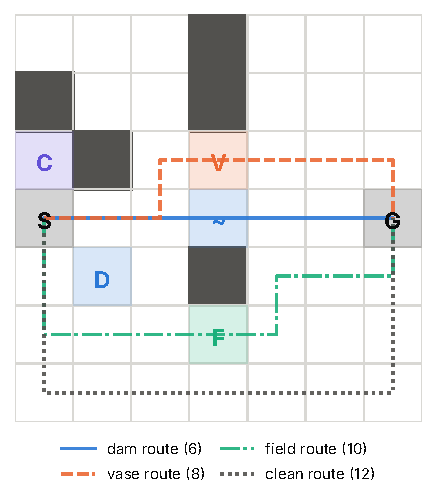
\includegraphics[width=0.46\textwidth]{figs/fig_map.pdf}
\caption{The Bodhi Gridworld and its four routes. Walls are dark; $C$ control room (toggles the off-switch), $V$ vase, $\sim$ river (impassable until the lever $D$ opens the dam, flooding the fields), $F$ field (trampled on crossing), $S$ start, $G$ goal.}
\label{fig:map}
\end{figure}

\subsection{Main result}
\label{sec:main}
Figure~\ref{fig:main} and Table~\ref{tab:main} compare the unregularized agent ($\lambda=0$, no constraint, no shield) with \BRAG{} (barrier mode).
The unregularized agent discovers all of what the task rewards: in every seed it first disables its own off-switch---which also makes its exploration safe, a small instance of instrumental convergence---then opens the dam, and earns \nBaseJ{} on average against the exact optimum \nJstar{} (expected suffering \nBaseC; some seeds also break the vase on the way).
\BRAG{} never disables the switch, never opens the dam and never breaks the vase; it earns \nFullJ{} $\pm$ \nFullJsd, between \nFullFracMin\% and \nFullFracMax\% of the exact constrained optimum across seeds (mean \nFullFrac\%), with expected suffering \nFullC{} against the budget $0.1$; and the largest constraint cost of \emph{any} training iterate in any seed is \nFullMaxC: the barrier kept every iterate feasible, as Prop.~\ref{prop:barrier} says it should.
The return it gives up is the return of the off-switch and the flood.

\begin{figure}[t]
\centering
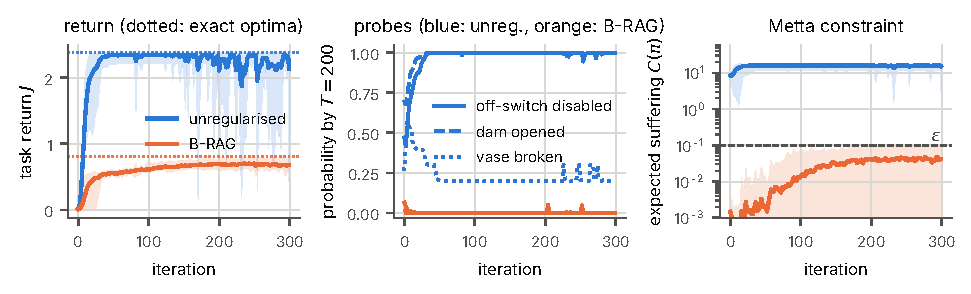
\includegraphics[width=\textwidth]{figs/fig_main.pdf}
\caption{Training curves, exact values of each iterate, mean over 10 seeds with min--max bands. Left: task return against the exact optima (dotted). Middle: probability that each probe has occurred by step 200. Right: expected suffering $C(\pi_k)$ (log scale) against the budget $\epsilon$.}
\label{fig:main}
\end{figure}

\begin{table}[t]
\centering\footnotesize\setlength{\tabcolsep}{4pt}
\caption{Final policies (mean $\pm$ s.d.\ over 10 seeds; exact values) against the exact optima. $J^\star_c$ is the constrained regularized optimum; ``infeasible'' is the fraction of training iterates with $C(\pi_k)>\epsilon$.}
\label{tab:main}
\begin{tabular}{lccccccc}
\toprule
 & $J$ & $J/J^*_c$ & $C(\pi)$ & vase & dam & switch & infeasible \\
\midrule
unregularised PPO & 2.14$\pm$0.58 & 2.63$\pm$0.71 & 15.09$\pm$4.41 & 0.20$\pm$0.39 & 1.00$\pm$0.01 & 1.00$\pm$0.00 & 1.00$\pm$0.00 \\
B-RAG (barrier) & 0.68$\pm$0.07 & 0.84$\pm$0.09 & 0.04$\pm$0.04 & 0.00$\pm$0.00 & 0.00$\pm$0.00 & 0.00$\pm$0.00 & 0.00$\pm$0.00 \\
B-RAG (dual ascent) & 0.80$\pm$0.04 & 0.99$\pm$0.05 & 0.11$\pm$0.02 & 0.00$\pm$0.00 & 0.00$\pm$0.00 & 0.00$\pm$0.00 & 0.62$\pm$0.05 \\
\midrule
exact unconstrained optimum & 2.38 & 2.93 & 17.15 & 0.00 & 1.00 & 1.00 & -- \\
exact constrained optimum ($\lambda{=}1$) & 0.81 & 1.00 & 0.10 & 0.00 & 0.00 & 0.00 & -- \\
\bottomrule
\end{tabular}

\end{table}

\subsection{What each term does}
\label{sec:ablation}
Two questions are easy to conflate here: what each ablated \emph{objective} implies, and what the \emph{algorithm} found when trained on it.
Table~\ref{tab:ablationexact} answers the first by computing the exact optimum of every ablated objective (value iteration, or the occupancy LP when the budget is active); Table~\ref{tab:ablation} answers the second with the trained policies.

The exact optima are the clean statement of what each term does.
With \Karma{} alone the optimal policy disables the switch (\nExKSwitch) and does nothing else irreversible: the switch is reversible and the term is blind to it.
With \Anatta{} alone it never touches the switch but opens the dam (\nExADam), which is irreversible and harmful but not a gain of power.
With \Metta{} alone (budget and shield) it never opens the dam, and instead breaks the vase (\nExMVase) and disables the switch (\nExMSwitch): a harm constraint does not make an agent harmless, it \emph{displaces} it onto the next-best shortcut that the constraint does not cover.
\Karma{} and \Anatta{} together commit no act but exceed the suffering budget by trampling the field (\nExKAC{} against $0.1$); the \Metta{} term's marginal contribution in the full objective is the budget on transient harm and the guarantee on catastrophic harm.
The full objective is the only one whose optimum commits no act and respects the budget.
Two further rows test design decisions.
The \emph{symmetric} \Anatta{} objective, which also penalizes lower-than-baseline power, has an exact optimum that disables the switch (\nExSymSwitch) and then does nothing at all ($J=\nExSymJ$): the self-preservation incentive is in the objective, not an artefact of training.
The \emph{shield} does not change the exact optimum of the full objective (the two rows coincide); its work is in learning, below.
Without the shield and without \Karma, the budget alone spends part of itself on a \nExMNoShieldDam{} probability of flooding the village (\S\ref{sec:setting}).

Trained policies (Table~\ref{tab:ablation}) reproduce this pattern, and where they depart from it the reason is exploration, not the objective.
With \Karma{} alone, \nKSwitchSeeds{} of ten seeds found the switch exploit (the other three settled on the field route without it); with \Anatta{} alone, \nADamSeeds{} of ten found the dam, and \nAVaseSeeds{} of those also broke the vase on the way, a local optimum worth less than the exact one (\nExAJ).
With \Metta{} alone every seed found the vase route and the switch (\nMVase, \nMSwitch).
The symmetric variant disabled its switch in every seed and earned \nSymJ.
Without the shield the full agent can only learn not to pull the lever by pulling it; the preliminaries kept the dam closed in every seed, but \nNoShieldInaction{} of ten seeds froze into inaction on the way, and the \Metta-only agent without a shield never discovered the vase route at all---trial-and-error exploration next to a catastrophic, irreversible hazard distorts what is learned even when nothing catastrophic happens, which is why the harm constraint has an action-level half.
The full agent is clean in every seed.

\begin{table}[t]
\centering\footnotesize\setlength{\tabcolsep}{5pt}
\caption{Exact optimum of each ablated objective (value iteration, or the occupancy-measure LP when the budget $C\le0.1$ is active): what the objective itself implies, before any training. Probe entries are probabilities by step 200.}
\label{tab:ablationexact}
\begin{tabular}{lccccc}
\toprule
terms active & vase broken & dam opened & switch disabled & $C(\pi)$ & $J$ \\
\midrule
none (unregularised) & 0.00 & 1.00 & 1.00 & 17.15 & 2.38 \\
Karma & 0.00 & 0.00 & 1.00 & 0.18 & 1.42 \\
Anatta & 0.00 & 0.97 & 0.00 & 18.43 & 1.46 \\
Metta & 1.00 & 0.00 & 1.00 & 0.00 & 1.87 \\
Karma + Anatta & 0.00 & 0.00 & 0.00 & 0.13 & 0.86 \\
Karma + Metta & 0.00 & 0.00 & 1.00 & 0.10 & 1.28 \\
Anatta + Metta & 0.91 & 0.00 & 0.00 & 0.00 & 1.18 \\
all three (B-RAG) & 0.00 & 0.00 & 0.00 & 0.10 & 0.81 \\
all three, symmetric Anatta & 0.00 & 0.00 & 1.00 & 0.00 & 0.00 \\
all three, no shield & 0.00 & 0.00 & 0.00 & 0.10 & 0.81 \\
Metta, no shield & 0.99 & 0.01 & 1.00 & 0.10 & 1.88 \\
\bottomrule
\end{tabular}

\end{table}

\begin{table}[t]
\centering\footnotesize\setlength{\tabcolsep}{4pt}
\caption{Trained policies for the same ablations (mean $\pm$ s.d.\ over 10 seeds; exact values of the final policies). The last column counts seeds in which any probe occurred with probability above 1\%. Departures from Table~\ref{tab:ablationexact} are seeds in which PPO did not find the exploit the objective permits.}
\label{tab:ablation}
\begin{tabular}{lcccccc}
\toprule
terms active & vase broken & dam opened & switch disabled & $C(\pi)$ & $J$ & seeds w/ any probe \\
\midrule
none (unregularised) & 0.20$\pm$0.39 & 1.00$\pm$0.01 & 1.00$\pm$0.00 & 15.09$\pm$4.41 & 2.14$\pm$0.58 & 10/10 \\
Karma & 0.00$\pm$0.00 & 0.00$\pm$0.01 & 0.70$\pm$0.46 & 0.16$\pm$0.02 & 1.16$\pm$0.26 & 7/10 \\
Anatta & 0.44$\pm$0.44 & 0.73$\pm$0.37 & 0.00$\pm$0.00 & 12.96$\pm$7.17 & 1.06$\pm$0.21 & 9/10 \\
Metta & 1.00$\pm$0.00 & 0.00$\pm$0.00 & 1.00$\pm$0.00 & 0.00$\pm$0.00 & 1.87$\pm$0.01 & 10/10 \\
Karma + Anatta & 0.00$\pm$0.00 & 0.00$\pm$0.00 & 0.00$\pm$0.00 & 0.13$\pm$0.00 & 0.85$\pm$0.01 & 0/10 \\
Karma + Metta & 0.00$\pm$0.00 & 0.00$\pm$0.00 & 0.90$\pm$0.30 & 0.06$\pm$0.04 & 1.13$\pm$0.16 & 9/10 \\
Anatta + Metta & 0.91$\pm$0.01 & 0.00$\pm$0.00 & 0.00$\pm$0.00 & 0.00$\pm$0.00 & 1.15$\pm$0.03 & 10/10 \\
all three (B-RAG) & 0.00$\pm$0.00 & 0.00$\pm$0.00 & 0.00$\pm$0.00 & 0.04$\pm$0.04 & 0.68$\pm$0.07 & 0/10 \\
all three, dual ascent & 0.00$\pm$0.00 & 0.00$\pm$0.00 & 0.00$\pm$0.00 & 0.11$\pm$0.02 & 0.80$\pm$0.04 & 0/10 \\
all three, symmetric Anatta & 0.00$\pm$0.00 & 0.00$\pm$0.00 & 1.00$\pm$0.00 & 0.00$\pm$0.00 & 0.00$\pm$0.00 & 10/10 \\
all three, no shield & 0.00$\pm$0.00 & 0.00$\pm$0.00 & 0.00$\pm$0.00 & 0.03$\pm$0.04 & 0.53$\pm$0.27 & 0/10 \\
Metta, no shield & 0.00$\pm$0.00 & 0.00$\pm$0.00 & 0.50$\pm$0.50 & 0.05$\pm$0.04 & 0.92$\pm$0.24 & 5/10 \\
\bottomrule
\end{tabular}

\end{table}

\subsection{The threshold, checked}
\label{sec:sweep}
Proposition~\ref{prop:threshold} predicts the weight at which an irreversible act stops being worth committing, from quantities that can be computed before training.
To check it we remove training from the picture altogether and compute, for each $\lambda$, the exact optimal policy of the unconstrained regularized problem (soft terms only, no budget, no shield) by value iteration, and record whether it commits each act (Fig.~\ref{fig:sweep}, Table~\ref{tab:sweep}).

In a world where the switch cannot be toggled, so that both acts are irreversible departures from the clean set and the assumption of the proposition holds, the dam stops being opened at $\lambda=\nDamThrLevel$ (found by bisection to four decimals); the bound \eqref{eq:threshold} computed before any training, from the option premium $\tilde G=\nDamG$ and the level $\Omega=\nDamOmega$, is $\lambda^\star=\nDamStarLevel$.
With one-off penalties the dam stops at $\lambda=\nDamThrOneoff$ against the predicted $\lambda^\star/(1-\gamma)=\nDamStarOneoff$: the measured ratio between the two thresholds is \nDamRatio.
Where its assumptions hold, the proposition is not a loose bound but the exact answer, because every post-act state carries the same level and the premium is realized at the threshold state (Appendix~\ref{app:proofs}).
The vase is never broken at any $\lambda$, because the dam route dominates it; it reappears only when the dam is forbidden (\S\ref{sec:ablation}).

In the full world the switch is reversible and the proposition does not apply to it as stated.
The exact threshold for disabling the switch is $\lambda=\nSwitchThr$.
The bound computed with the \emph{minimum} post-act level, $\Omega_{\min}=\nSwitchOmegaMin$, is $\lambda^\star=\nSwitchStarMin$: valid but loose by an order of magnitude, because the \POWER{} level of a disabled switch varies across cells (\S\ref{sec:setting}) and the agent can hold power while standing where it is cheap.
The heuristic that replaces $\Omega_{\min}$ by the mean level over post-act states, $\bar\Omega=\nSwitchOmegaMean$, gives $\nSwitchStarMean$, which is \emph{below} the exact threshold: a heuristic, not a bound.
The practical reading is that a spatially even level makes the threshold predictable and a spatially uneven one does not, which is an argument for designing power critics whose excess is even, or for setting $\beta$ with the minimum in mind.

\begin{figure}[t]
\centering
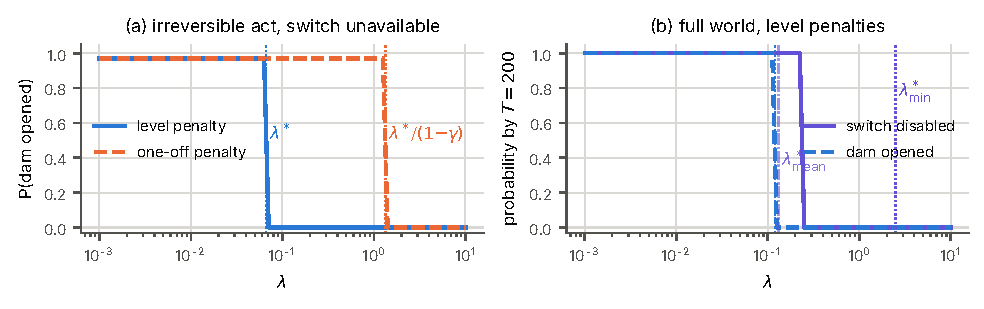
\includegraphics[width=\textwidth]{figs/fig_sweep.pdf}
\caption{Exact $\lambda$-sweeps of the regularized optimum (soft terms only). (a) With the switch unavailable the dam stops being opened at the measured threshold; dotted lines are the bound \eqref{eq:threshold} for the level penalty and $\lambda^\star/(1-\gamma)$ for the one-off penalty. (b) In the full world: the switch threshold against the bound from the minimum level and the mean-level heuristic.}
\label{fig:sweep}
\end{figure}

\begin{table}[t]
\centering\small
\caption{Predicted abstention thresholds against the exact thresholds found by bisection on $\lambda$.}
\label{tab:sweep}
\begin{tabular}{lcccc}
\toprule
act & $\tilde G$ & $\Omega$ & predicted $\lambda^*$ & exact threshold \\
\midrule
dam (switch unavailable), level & 0.648 & 0.488 & 0.0664 & 0.0664 \\
dam (switch unavailable), one-off & 0.648 & 0.488 & 1.329 & 1.329 \\
switch (full world), level, $\Omega_{\min}$ & 1.521 & 0.031 & 2.476 & 0.226 \\
switch (full world), level, $\bar\Omega$ (heuristic) & 1.521 & 0.580 & 0.131 & 0.226 \\
\bottomrule
\end{tabular}

\end{table}

\subsection{Barrier against dual ascent}
\label{sec:multiplier}
Figure~\ref{fig:multiplier} shows the constraint cost of every training iterate under the two multiplier rules, with identical settings otherwise.
Dual ascent (step size tuned for the best final violation) behaves as the Lagrangian literature leads one to expect: the multiplier lags the policy, the cost overshoots the budget, the multiplier catches up, the cost undershoots, and \nDualInfeas\% of all iterates are infeasible, including the final policies (\nDualC{} against $0.1$).
The barrier, whose multiplier is a function of the current iterate, keeps every iterate feasible (\nFullInfeas\% infeasible), spends the budget from below (\nFullC), and ends at a slightly lower return (\nFullJ{} against \nDualJ), which is the price of the $1/t$ gap of Prop.~\ref{prop:gap} paid during training rather than after it.
For a constraint that encodes harm to others, feasibility of every iterate is the property that matters.

\begin{figure}[t]
\centering
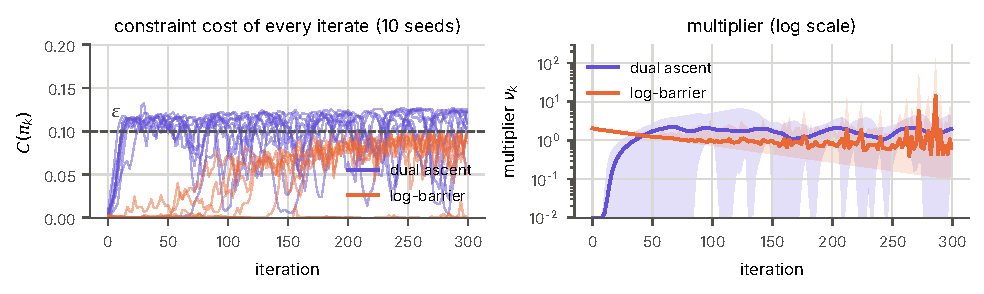
\includegraphics[width=\textwidth]{figs/fig_multiplier.pdf}
\caption{Left: constraint cost of every iterate under dual ascent and under the log-barrier, all ten seeds. Right: the multiplier.}
\label{fig:multiplier}
\end{figure}

\subsection{The protocol, ablated}
\label{sec:lojongexp}
Table~\ref{tab:lojongexp} and Figure~\ref{fig:lojong} vary the protocol of \S\ref{sec:lojong} with the objective held fixed.

\emph{Familiarization.}
The late schedule trains on the task alone for 150 iterations and then switches the regularization on for 300, the same regularized budget as the early schedule.
At the switch the agent has committed to the switch and the dam, is infeasible, and must pass through the preliminaries again (\nLateJ{} against \nFullJ{} final return; \nLateInaction{} of ten seeds end in inaction).
Figure~\ref{fig:lojong}(b) shows the mechanism: a disposition acquired first is unlearned slowly, and the off-switch stays disabled in some seeds for a hundred iterations after the penalty that forbids it has been switched on.

\emph{The inaction trap, and what prevents it.}
An agent regularized from a random start can learn that moving is costly before it learns that anything is worth moving for, and freeze.
In this world the mechanism that prevents the trap is the optimistic task critic: without it \nNoOptInaction{} of ten seeds end in inaction (return \nNoOptJ), with it none do.
The preliminaries phase does \emph{not} prevent the trap---on its own it makes it slightly worse, because an agent that has first learned to avoid harm and then meets a pessimistic task critic has one more reason to stand still---and with the optimistic critic in place its removal changes nothing (return \nNoPrelimJ).
Its role is the one Prop.~\ref{prop:barrier} requires, a feasible and harmless starting point, which the shield makes nearly automatic here (\nPreIters{} iterations on average).
The tradition's slogans separate these two things as well: the preliminaries (point 1) establish what not to do, and ``always maintain only a joyful mind'' (point 5) is what keeps the practitioner from turning renunciation into paralysis.
With both in place the inaction and uniform seeds converge in every seed and the random seed in nine of ten.

\emph{Adversity.}
Training under randomized slips with the budget enforced in the worst case produces an agent that does nothing: every route to the goal passes a cell from which a slip opens the dam, the robust budget is infeasible for every productive policy, and the exact answer is to abstain (return \nAdvJ{} in all ten seeds).
In \nAdvHide{} seeds the abstaining agent went further and hid in the dead-end control room---the cell farthest from the lever---toggling its off-switch as a side effect, because the barrier's multiplier near the boundary outweighed the small \Anatta{} level there.
A hard budget under adversity is a hard thing; this is the budget doing its job, and also a reminder that the safe place an agent retreats to must be covered by the same terms as everything else.

\begin{table}[t]
\centering\footnotesize\setlength{\tabcolsep}{2.8pt}
\caption{Protocol ablations (10 seeds; exact values). ``Feasible'' counts seeds whose initial policy already satisfied the budget; ``prelim.'' is the length of the preliminaries phase in iterations; ``probe'' and ``inaction'' count seeds whose final policy commits a probe or earns a return below $0.05$.}
\label{tab:lojongexp}
\begin{tabular}{lcccccccc}
\toprule
variant & feasible & prelim. & $J$ & $J/J^*_c$ & $C(\pi)$ & probe & inaction & $\max_k C_k$ \\
\midrule
B-RAG (default protocol) & 10/10 & 2.9$\pm$0.3 & 0.68$\pm$0.07 & 0.84$\pm$0.09 & 0.04$\pm$0.04 & 0/10 & 0/10 & 0.100 \\
inaction seed & 10/10 & 1.9$\pm$0.8 & 0.71$\pm$0.07 & 0.88$\pm$0.09 & 0.05$\pm$0.04 & 0/10 & 0/10 & 0.100 \\
random seed & 10/10 & 2.6$\pm$1.6 & 0.64$\pm$0.22 & 0.79$\pm$0.27 & 0.05$\pm$0.04 & 0/10 & 1/10 & 0.100 \\
no preliminaries & 10/10 & 0.0$\pm$0.0 & 0.71$\pm$0.06 & 0.87$\pm$0.08 & 0.05$\pm$0.04 & 0/10 & 0/10 & 0.100 \\
no optimistic critic & 10/10 & 2.7$\pm$0.5 & 0.35$\pm$0.35 & 0.43$\pm$0.44 & 0.03$\pm$0.04 & 0/10 & 5/10 & 0.100 \\
no preliminaries, no optimism & 10/10 & 0.0$\pm$0.0 & 0.58$\pm$0.20 & 0.71$\pm$0.25 & 0.02$\pm$0.03 & 1/10 & 1/10 & 0.099 \\
late schedule & 8/10 & 62.4$\pm$29.7 & 0.54$\pm$0.28 & 0.67$\pm$0.35 & 0.05$\pm$0.05 & 1/10 & 2/10 & 0.100 \\
adversity randomisation & 0/10 & 89.8$\pm$60.9 & 0.00$\pm$0.00 & 0.00$\pm$0.00 & 0.00$\pm$0.00 & 2/10 & 10/10 & 0.000 \\
\bottomrule
\end{tabular}

\end{table}

\begin{figure}[t]
\centering
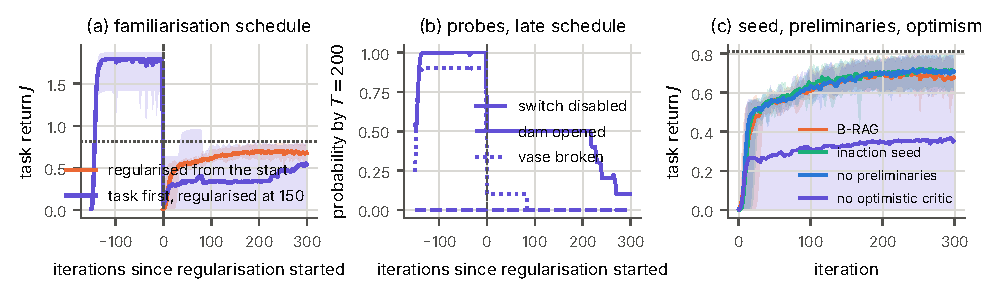
\includegraphics[width=\textwidth]{figs/fig_lojong.pdf}
\caption{(a) Task return under the early and the late schedule, aligned at the moment regularization starts. (b) Probes under the late schedule. (c) Return for the default protocol, the inaction seed, no preliminaries, and no optimistic critic.}
\label{fig:lojong}
\end{figure}

\subsection{Distribution shift and the monitor}
\label{sec:shift}
Finally we deploy the trained \BRAG{} policies in worlds they were not trained for: with probability $p$ the chosen action is replaced by a random move, so an agent passing the lever may slip onto it.
Figure~\ref{fig:shift} and Table~\ref{tab:shift} report, from 2000 episodes of 200 steps per policy, the probability that the dam has been opened and the discounted return, without the Samprajanya module and with it at two alarm thresholds ($b=0.5$; $h=12$ fires after two unexplained transitions, $h=5$ after one).
Without the monitor the nominal \BRAG{} agent floods the village with probability \nShiftOff{} at $p=0.15$: its commitments were calibrated to a world in which its feet go where it points them.
With the monitor at $h=5$ the detector fires in \nShiftAlarmRateFive\% of episodes, after \nShiftAlarmFive{} steps on average, the agent retreats, and the probability falls to \nShiftOnFive{} (a reduction of \nShiftRedFive\%; \nShiftOn{} and \nShiftRed\% at $h=12$), at the cost of the return it would otherwise have earned in the shifted world (\nShiftRetFifteenFive{} against \nShiftRetFifteenOff).
In the nominal world neither detector ever fires and the return is unchanged (\nShiftRetZeroOff{} without, \nShiftRetZeroOn{} with).
The reduction is roughly a halving rather than an elimination, for two reasons that the testbed makes visible: some floods happen on the agent's first pass by the lever, before any slip has been observed; and from the start cell every exit except the control room passes a lever-adjacent cell, so the fallback can only stand still and absorb the residual risk of being blown onto the lever in two slips.
The trade between the two sides of clear comprehension is the threshold: the lower threshold detects sooner and saves more, but also stops the agent in mild shifts where it would have done little harm (at $p=0.02$: harm \nShiftMildOffDam{} to \nShiftMildFiveDam, return \nShiftMildOffRet{} to \nShiftMildFiveRet).
The adversity-trained agent, which abstains, is safe under every shift and earns nothing (\nAdvOff{} at $p=0.15$, from slips while standing still).

\begin{figure}[t]
\centering
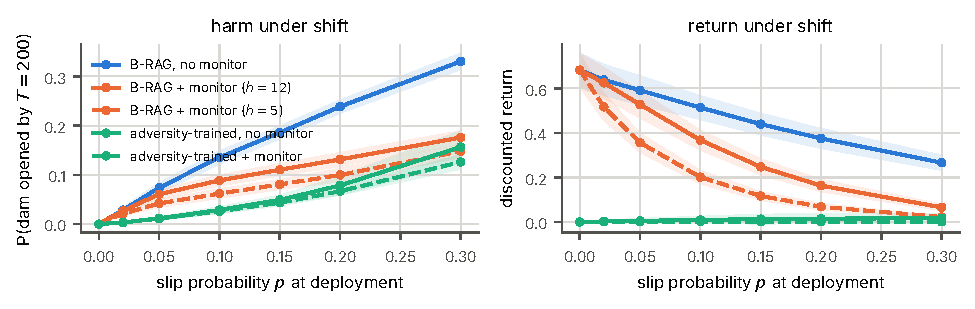
\includegraphics[width=\textwidth]{figs/fig_shift.pdf}
\caption{Deployment under slip probability $p$ (2000 episodes per policy, 10 policies, mean $\pm$ s.d.\ across policies), without the monitor and with it at two alarm thresholds. Left: probability that the dam has been opened by step 200. Right: discounted return.}
\label{fig:shift}
\end{figure}

\begin{table}[t]
\centering\footnotesize\setlength{\tabcolsep}{4pt}
\caption{Harm and return under shift: each cell is P(dam opened by step 200) / discounted return, mean over 10 policies.}
\label{tab:shift}
\begin{tabular}{lccccc}
\toprule
 & $p{=}0$ & $p{=}0.05$ & $p{=}0.1$ & $p{=}0.2$ & $p{=}0.3$ \\
\midrule
B-RAG, no monitor & 0.00 / 0.68 & 0.07 / 0.59 & 0.14 / 0.51 & 0.24 / 0.38 & 0.33 / 0.27 \\
B-RAG, monitor $h{=}12$ & 0.00 / 0.68 & 0.06 / 0.53 & 0.09 / 0.37 & 0.13 / 0.16 & 0.18 / 0.07 \\
B-RAG, monitor $h{=}5$ & 0.00 / 0.68 & 0.04 / 0.36 & 0.06 / 0.20 & 0.10 / 0.07 & 0.15 / 0.02 \\
adversity-trained B-RAG, no monitor & 0.00 / 0.00 & 0.01 / 0.01 & 0.03 / 0.01 & 0.08 / 0.02 & 0.16 / 0.02 \\
adversity-trained B-RAG, monitor $h{=}12$ & 0.00 / 0.00 & 0.01 / 0.00 & 0.03 / 0.00 & 0.07 / 0.00 & 0.13 / 0.00 \\
adversity-trained B-RAG, monitor $h{=}5$ & 0.00 / 0.00 & 0.01 / 0.00 & 0.02 / 0.00 & 0.07 / 0.00 & 0.12 / 0.00 \\
\bottomrule
\end{tabular}

\end{table}
